\section{Results and Discussion}
\label{Chap:Al/Vac:section:RD}
\subsection{Cluster Searching Algorithm}

In order to better analyzing our results, we have to use a visualization method to characterize clusters. A cluster is a set of connected atoms, each of which is within the range of one or more other atoms from the same cluster. Thus, any two atoms from the same cluster are connected by a continuous path consisting of steps fulfilling the selected neighboring criterion. Adversely, two atoms are not considered in the same cluster if there is no continuous path on the neighbor network leading from one particle to the other. We choose between the distance-based neighbor criterion, in which case two atoms are considered neighbors if they are within the neighbor list of each other. However, in our case, all the atoms are on lattice, so the method described above does not work. It will simply find one huge cluster containing all the atoms. Therefore, we use the method described in Algorithm. \ref{algo:cluster}. We show one typical results in Fig. \ref{Chap:Al/Vac:fig:illu_cluster}. The only top ten clusters are shown. And as you can see, dark red and orange clusters are almost connected. They share one Al atom in common. In that case we treat them as two clusters. Otherwise, if Al atoms are treated like bridges, then most of the atoms in the supercell will be connected as one huge cluster, which is not desired.


\begin{figure}[!htb]
  \centering
  \begin{minipage}{.75\linewidth}
    \begin{algorithm}[H]
      \caption{Cluster Searching Algorithm}\label{algo:cluster}
      \begin{algorithmic}[1]
        \State remove all the solvent atoms (Al for example).
        \State assign an initial cluster id, ($cid = -1$), to all the atoms.
        \State set $count = 0$.
        \For {i in all the solute atoms}
          \If {$cid_i = -1$}
            \State set $cid_i = count$.
            \State \ac{BFS} in the neighbor list of atom i to find other solute atoms if cluster size is greater than $size_{critical}$ and set their $cid = count$.
            \State add their first nearest neighbor solvent atoms (Al for example) back if the solvent atom have more than $bond_{critical}$ solute first nearest neighbors and set their $cid = count$.
            \State $count += 1$.
          \EndIf
        \EndFor
        \State then clusters can be sorted according to any customized methods, by cluster size, element ratios for examples.
      \end{algorithmic}
    \end{algorithm}
  \end{minipage}
\end{figure}


\begingroup
\begin{figure}[!ht]
  \centering
  \subfigure[]{\includegraphics[width=0.49\linewidth]{Chap5/plots/cluster_illu_1.png}}
  \subfigure[]{\includegraphics[width=0.45\linewidth]{Chap5/plots/cluster_illu_2.png}}
\caption[Atomistic pictures of top 10 clusters by size via cluster searching algorithm.]{Atomistic pictures of top 10 clusters by size via cluster searching algorithm. (a) Atomistic pictures of clusters coloring in atom species. Light green, dark green, and red atoms are Al, Mg, and Zn, respectively. (b) Atomistic pictures of clusters coloring in cluster id. The color mapping from dark blue to red is ranked by the cluster size in descending order.}
\label{Chap:Al/Vac:fig:illu_cluster}
\end{figure}
\endgroup


\subsection{Searching for Potential Elements that Can Slow Down Early Stage Nucleation}
\label{Chap:Al/Vac:pseudo}
Similar to the idea of searching ``anchor'' elements in Chap. \ref{Chap:Ag/ZnO:section:anchor}, we will first use \ac{KMC} simulation with some pseudo-atoms (denoted as ``X'') to study their effects on the early stage clustering. In this study, we have Al atoms as solvent atoms, and Mg, Zn atoms as solute atoms. To tune the properties of pseudo atoms, we can change the effects of different elements on vacancy diffusion barriers to the pseudo-atoms, as well as barriers to other elements. We leverage this by adding an offset to the diffusion barrier calculated from \ac{NN} model via Equation. \ref{Chap:Al/Vac:eq:offset} . The amount of the offset is determined by counting first neighbor bonding of X-Al, X-Mg, and X-Zn, via Equation. \ref{Chap:Al/Vac:eq:offset_calculation}:
\begin{subequations}
\begin{align}
{E_a}^{actual} & = {E_a}^{NN} + \textit{offset} \label{Chap:Al/Vac:eq:offset} \\
\textit{offset} & = \sum_{i\in\{Al, Mg, Zn\}} \varepsilon_{i-X} * ( n_{i-X}^{final} - n_{i-X}^{init}) \label{Chap:Al/Vac:eq:offset_calculation}
\end{align}
\end{subequations}
where ${E_a}^{NN}$ is the energy obtained by the neural network prediction of treating element ``X'' as the solvent element Al, the summation is confined to first nearest-neighbors of the vacancy and of the jumping atom, $\varepsilon_{i-X}$ represents the amount of different pairs' effects on the diffusion barrier offset, and $n_{i-X}$ is the number of first nearest neighbor $i-X$ pairs. For example, if $\varepsilon_{Al-X} = 0.01$ that means increasing an Al-X pair will increase the diffusion barrier by a positive 0.01 eV.


The right hand side of Equation. \ref{Chap:Al/Vac:eq:offset} can be divided into two parts. The first part, which is \ac{NN} potential part, can be seen as a more comprehensive bond counting model \cite{soisson1996monte} base on the pair interactions of Al-Al, Al-Mg, Al-Zn, and Mg-Zn, plus cross interactions or higher odered angular contributions. And the second part of the RHS is can be seen as first order bond counting of Al-X, Mg-X, and Zn-X. As a qualitative study, first order pair-wise interaction of the unknown pseudo-atoms should be sufficient. If we rearrange Equation. \ref{Chap:Al/Vac:eq:offset}, we will have:
\begin{subequations}
\begin{align}
{E_a}^{actual} & = \sum_{i, j \in\{Al, Mg, Zn, X\} \& i \neq j} \varepsilon_{i-j} * ( n_{i-j}^{final} - n_{i-j}^{init}) + \textit{H.O.T.(Al, Mg, Zn)} \label{Chap:Al/Vac:eq:rearrange}
\end{align}
\end{subequations}
where $H.O.T$ is the higher order term, such as bond angles. Then the target is to find an element ``X'' that can change the diffusion barrier of Vac-i by roughly the amount of $\varepsilon_{i-X}$, where $i \in \{Al, Mg, Zn\}$.


\begin{table}[!htbp]
\centering
\caption[Sensitivity analysis of different $\varepsilon_{i-X}$.]{Sensitivity analysis of different $\varepsilon_{i-X}$. In the table, the number of different element types are listed using $size_{critical}$ of 3(4) and $bond_{critical}$ of 3(4).}
\label{Chap:Al/Vac:tab:pseudo1}
\begin{tabular}{cccccccc}
\\
\hline
\hline
setup & $\varepsilon_{Al-X}$  & $\varepsilon_{Mg-X}$  & $\varepsilon_{Zn-X}$ & Al counts & Mg counts & Zn counts & pseudo counts\\
\hline
0 &  0.00    &  0.00       &  0.00 & 1078(230) & 588(421)  &  737(524)  & 11(4)                \\
1 &  0.05    &  0.00       &  0.00 & 1229(270) &  689(434) &   778(549) & 0(0)                \\
2 & -0.05    &  0.00       &  0.00 & 1407(312) & 922(753)  & 1017(871)  & 406(252)                \\
3 &  0.05    &  0.05       &  0.00 & 1442(353) & 1121(919) & 794(620)   & 292(171)                \\
4 &  0.00    & -0.05       &  0.00 & 1012(215) &  588(407) &  638(463)  & 5(1)                \\
5 &  0.00    &  0.00       &  0.05 & 1407(395) & 522(407)  & 1325(1164) & 385(253)                \\
6 &  0.00    &  0.00       & -0.05 & 1042(222) &  590(363) &  730(489)  & 3(0)                \\

\hline
\hline
\end{tabular}
\end{table}


To setup the simulation for sensitivity tests, we use \ac{LSKMC} method with $step_{critical}$ of 25,000 steps and $E_{critical}$ of 0.3 eV. After around 5 $\sim$ 6 seconds simulation, we can already tell the differences of cluster size obviously. As discussed above, we tuned parameters of $\varepsilon_{i-X}$ for $i \in {Al, Mg, Zn}$. Detailed setup is listed in Table. \ref{Chap:Al/Vac:tab:pseudo1}. And their corresponding final snapshots can be found in Fig. \ref{Chap:Al/Vac:fig:sens_Al}, Fig. \ref{Chap:Al/Vac:fig:sens_Mg}, and Fig. \ref{Chap:Al/Vac:fig:sens_Zn}, respectively. In order to achieve the target of finding a suitable element ``X'', we can use \ac{DFT} with \ac{NEB} to search for elements that can change the diffusion barrier of Vac-i by roughly the amount of $\varepsilon_{i-X}$, where $i \in \{Al, Mg, Zn\}$.


\newpage
\begingroup
\begin{figure}[!ht]
  \centering
  \subfigure[Al Mg Zn X]{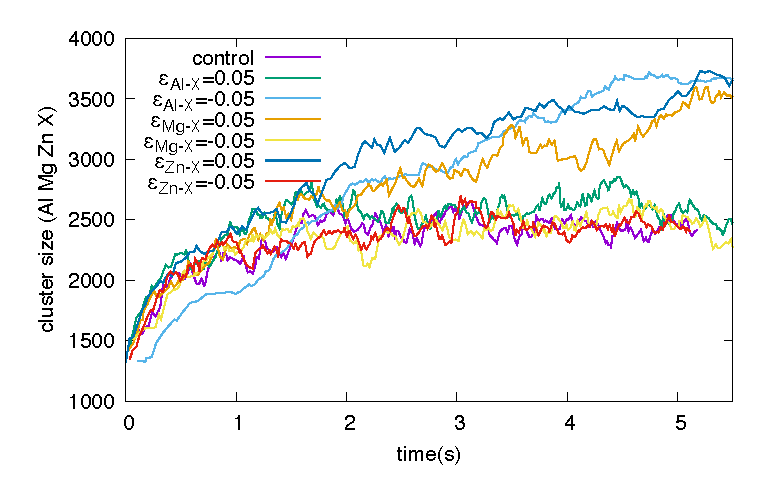
\includegraphics[width=0.8\linewidth]{Chap5/plots/size.eps}}
  \subfigure[Al Mg Zn]{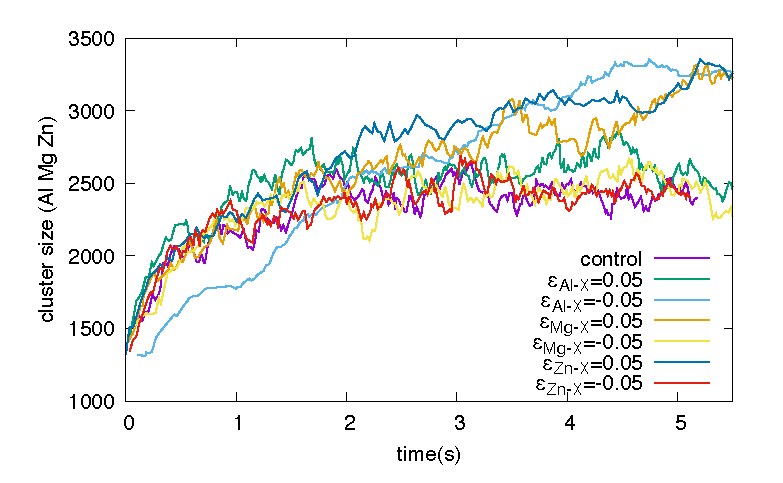
\includegraphics[width=0.8\linewidth]{Chap5/plots/size_noX.eps}}
\caption[Size changes of different clusters vs. time using $size_{critical}$ of 3 and $bond_{critical}$ of 3.]{Size changes of different clusters vs. time using $size_{critical}$ of 3 and $bond_{critical}$ of 3. Subplot. (a) is for all the atoms including pseudo atoms. (b) is for Al, Mg, and Zn only.}
\label{Chap:Al/Vac:fig:sens_cluster_size}
\end{figure}
\endgroup


\newpage
\begingroup
\begin{figure}[!ht]
  \centering
  \subfigure[cluster]{\includegraphics[width=0.8\linewidth]{Chap5/plots/cluster_id_jpg/00000.jpg}}
  \subfigure[species]{\includegraphics[width=0.8\linewidth]{Chap5/plots/element_jpg/00000.jpg}}
\caption[Atomistic pictures of 108,000 atoms for $\varepsilon_{Al-X}$ sensitivity test.]{Atomistic pictures of 108,000 atoms for control group, corresponding to setup \#0 in Table. \ref{Chap:Al/Vac:tab:pseudo1}. Subplot. (a) is colored by cluster size. The color mapping from dark blue to red is ranked by the cluster size in descending order. Subplot. (b) is colored by atom species. Light green, dark green, red, and blue atoms are Al, Mg, Zn, and pseudo atoms respectively.}
\label{Chap:Al/Vac:fig:sens_control}
\end{figure}
\endgroup


\newpage
\begingroup
\begin{figure}[!ht]
  \centering
  \subfigure[ratio of Al/(Mg+Zn)]{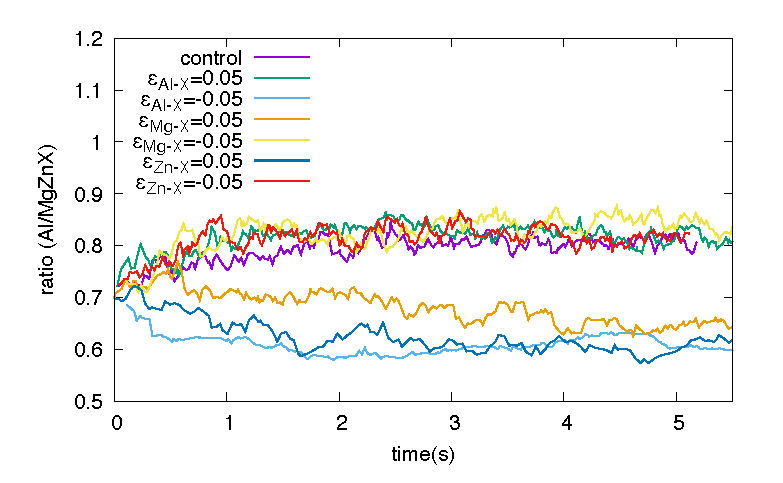
\includegraphics[width=0.8\linewidth]{Chap5/plots/ratio_Al-MgZnX.eps}}
  \subfigure[ratio of Mg/Zn]{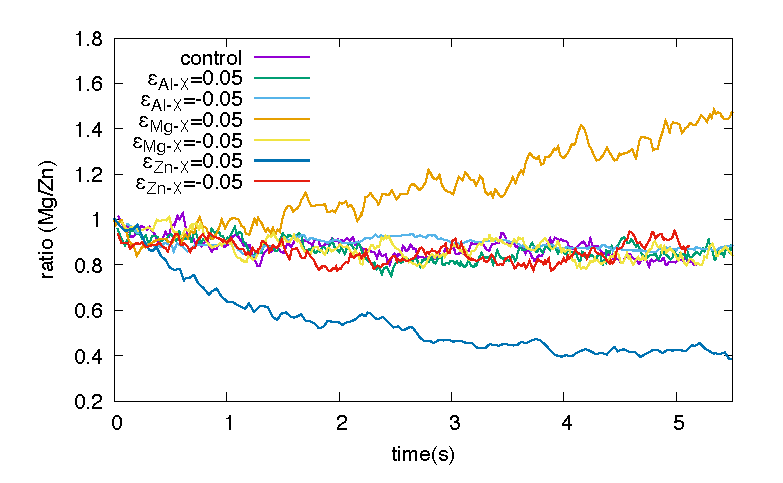
\includegraphics[width=0.8\linewidth]{Chap5/plots/ratio_Mg-Zn.eps}}
\caption[Ratio changes of different clusters vs. time using $size_{critical}$ of 3 and $bond_{critical}$ of 3.]{Ratio changes of different clusters vs. time using $size_{critical}$ of 3 and $bond_{critical}$ of 3. Subplot. (a) is for the ratio between all the Al atoms and the sum of Mg and Zn atoms in the clusters. (b) is for Mg and Zn ratio in the clusters.}
\label{Chap:Al/Vac:fig:sens_cluster_ratio}
\end{figure}
\endgroup


\newpage
\begingroup
\begin{figure}[!ht]
  \centering
  \subfigure[$\varepsilon_{Al-X} = 0.05$ cluster]{\includegraphics[width=0.49\linewidth]{Chap5/plots/cluster_id_jpg/00001.jpg}}
%   \subfigure[controlcluster]{\includegraphics[width=0.49\linewidth]{Chap5/plots/cluster_id_jpg/00000.jpg}}
  \subfigure[$\varepsilon_{Al-X} = -0.05$ cluster]{\includegraphics[width=0.49\linewidth]{Chap5/plots/cluster_id_jpg/00002.jpg}}
  \subfigure[$\varepsilon_{Al-X} = 0.05$ species]{\includegraphics[width=0.49\linewidth]{Chap5/plots/element_jpg/00001.jpg}}
%   \subfigure[control species]{\includegraphics[width=0.49\linewidth]{Chap5/plots/element_jpg/00000.jpg}}
  \subfigure[$\varepsilon_{Al-X} = -0.05$ species]{\includegraphics[width=0.49\linewidth]{Chap5/plots/element_jpg/00002.jpg}}
% \caption[Atomistic pictures of 108,000 atoms for $\varepsilon_{Al-X}$ sensitivity test.]{Atomistic pictures of 108,000 atoms for $\varepsilon_{Al-X}$ sensitivity test. (a), (d) : $\varepsilon_{Al-X} = 0.05$, which is setup \#1 in Table. \ref{Chap:Al/Vac:tab:pseudo1}. (b), (e) : setup \#0 in Table. \ref{Chap:Al/Vac:tab:pseudo1}. (c), (f) : $\varepsilon_{Al-X} = -0.05$, which is setup \#2 in Table. \ref{Chap:Al/Vac:tab:pseudo1}. (a), (b), and (c) are colored by cluster size. The color mapping from dark blue to red is ranked by the cluster size in descending order. (d), (e), and (f) are colored by atom species.  Light green, dark green, red, and blue atoms are Al, Mg, Zn, and pseudo atoms respectively.}
\caption[Atomistic pictures of 108,000 atoms for $\varepsilon_{Al-X}$ sensitivity test.]{Atomistic pictures of 108,000 atoms for $\varepsilon_{Al-X}$ sensitivity test. (a), (c) : $\varepsilon_{Al-X} = 0.05$, which is setup \#1 in Table. \ref{Chap:Al/Vac:tab:pseudo1}. (b), (d) : $\varepsilon_{Al-X} = -0.05$, which is setup \#2 in Table. \ref{Chap:Al/Vac:tab:pseudo1}. (a) and (c) are colored by cluster size. The color mapping from dark blue to red is ranked by the cluster size in descending order. (b) and (d) are colored by atom species. Light green, dark green, red, and blue atoms are Al, Mg, Zn, and pseudo atoms respectively.}
\label{Chap:Al/Vac:fig:sens_Al}
\end{figure}
\endgroup


\newpage
\begingroup
\begin{figure}[!ht]
  \centering
  \subfigure[$\varepsilon_{Mg-X} = 0.05$ cluster]{\includegraphics[width=0.49\linewidth]{Chap5/plots/cluster_id_jpg/00003.jpg}}
%   \subfigure[control]{\includegraphics[width=0.32\linewidth]{Chap5/plots/cluster_id_jpg/00000.jpg}}
  \subfigure[$\varepsilon_{Mg-X} = -0.05$ cluster]{\includegraphics[width=0.49\linewidth]{Chap5/plots/cluster_id_jpg/00004.jpg}} \\
  \subfigure[$\varepsilon_{Mg-X} = 0.05$ species]{\includegraphics[width=0.49\linewidth]{Chap5/plots/element_jpg/00003.jpg}}
%   \subfigure[control]{\includegraphics[width=0.32\linewidth]{Chap5/plots/element_jpg/00000.jpg}}
  \subfigure[$\varepsilon_{Mg-X} = -0.05$ species]{\includegraphics[width=0.49\linewidth]{Chap5/plots/element_jpg/00004.jpg}}
% \caption[Atomistic pictures of 108,000 atoms for $\varepsilon_{Mg-X}$ sensitivity test.]{Atomistic pictures of 108,000 atoms for $\varepsilon_{Mg-X}$ sensitivity test. (a), (d) : $\varepsilon_{Mg-X} = 0.05$, which is setup \#3 in Table. \ref{Chap:Al/Vac:tab:pseudo1}. (b), (e) : setup \#0 in Table. \ref{Chap:Al/Vac:tab:pseudo1}. (c), (f) : $\varepsilon_{Mg-X} = -0.05$, which is setup \#4 in Table. \ref{Chap:Al/Vac:tab:pseudo1}. (a), (b), and (c) are colored by cluster size. The color mapping from dark blue to red is ranked by the cluster size in descending order. (d), (e), and (f) are colored by atom species.  Light green, dark green, red, and blue atoms are Al, Mg, Zn, and pseudo atoms respectively.}
\caption[Atomistic pictures of 108,000 atoms for $\varepsilon_{Mg-X}$ sensitivity test.]{Atomistic pictures of 108,000 atoms for $\varepsilon_{Mg-X}$ sensitivity test. (a), (c) : $\varepsilon_{Mg-X} = 0.05$, which is setup \#3 in Table. \ref{Chap:Al/Vac:tab:pseudo1}. (b), (d) : $\varepsilon_{Mg-X} = -0.05$, which is setup \#4 in Table. \ref{Chap:Al/Vac:tab:pseudo1}. (a) and (c) are colored by cluster size. The color mapping from dark blue to red is ranked by the cluster size in descending order. (b) and (d) are colored by atom species. Light green, dark green, red, and blue atoms are Al, Mg, Zn, and pseudo atoms respectively.}
\label{Chap:Al/Vac:fig:sens_Mg}
\end{figure}
\endgroup

\newpage
\begingroup
\begin{figure}[!ht]
  \centering
  \subfigure[$\varepsilon_{Zn-X} = 0.05$ cluster]{\includegraphics[width=0.49\linewidth]{Chap5/plots/cluster_id_jpg/00005.jpg}}
%   \subfigure[control]{\includegraphics[width=0.32\linewidth]{Chap5/plots/cluster_id_jpg/00000.jpg}}
  \subfigure[$\varepsilon_{Zn-X} = -0.05$ cluster]{\includegraphics[width=0.49\linewidth]{Chap5/plots/cluster_id_jpg/00006.jpg}} \\
  \subfigure[$\varepsilon_{Zn-X} = 0.05$ species]{\includegraphics[width=0.49\linewidth]{Chap5/plots/element_jpg/00005.jpg}}
%   \subfigure[control]{\includegraphics[width=0.32\linewidth]{Chap5/plots/element_jpg/00000.jpg}}
  \subfigure[$\varepsilon_{Zn-X} = -0.05$ species]{\includegraphics[width=0.49\linewidth]{Chap5/plots/element_jpg/00006.jpg}}
% \caption[Atomistic pictures of 108,000 atoms for $\varepsilon_{Zn-X}$ sensitivity test.]{Atomistic pictures of 108,000 atoms for $\varepsilon_{Zn-X}$ sensitivity test. (a), (d) : $\varepsilon_{Zn-X} = 0.05$, which is setup \#5 in Table. \ref{Chap:Al/Vac:tab:pseudo1}. (b), (e) : setup \#0 in Table. \ref{Chap:Al/Vac:tab:pseudo1}. (c), (f) : $\varepsilon_{Zn-X} = -0.05$, which is setup \#6 in Table. \ref{Chap:Al/Vac:tab:pseudo1}. (a), (b), and (c) are colored by cluster size. The color mapping from dark blue to red is ranked by the cluster size in descending order. (d), (e), and (f) are colored by atom species.  Light green, dark green, red, and blue atoms are Al, Mg, Zn, and pseudo atoms respectively.}
\caption[Atomistic pictures of 108,000 atoms for $\varepsilon_{Zn-X}$ sensitivity test.]{Atomistic pictures of 108,000 atoms for $\varepsilon_{Zn-X}$ sensitivity test. (a), (c) : $\varepsilon_{Zn-X} = 0.05$, which is setup \#5 in Table. \ref{Chap:Al/Vac:tab:pseudo1}. (b), (d) : $\varepsilon_{Zn-X} = -0.05$, which is setup \#6 in Table. \ref{Chap:Al/Vac:tab:pseudo1}. (a) and (c) are colored by cluster size. The color mapping from dark blue to red is ranked by the cluster size in descending order. (b) and (d) are colored by atom species. Light green, dark green, red, and blue atoms are Al, Mg, Zn, and pseudo atoms respectively.}
\label{Chap:Al/Vac:fig:sens_Zn}
\end{figure}
\endgroup